\documentclass{article}
\title{Notes for: Algorithms for Inverse Reinforcement Learning}
\author{-- \thanks{paper: https://ai.stanford.edu/~ang/papers/icml00-irl.pdf}}
\date{\today}
\usepackage{graphicx}
\usepackage{amsfonts}

\begin{document}
    \maketitle
    
    \section{High Level and Motivation}

    \subsection{Problem}
    
    \begin{itemize}
        \item Normal reinforcement learning is the process of extracting an optimal policy for a given reward function in an environment.
        \item Inverse reinforcement learning is the process of extracting a reward function from an environment given observed \textbf{optimal behavior}.
    \end{itemize}
    
    \subsection{Example}
    You are able to observe an agent's actions as it tackles a modified version of the Mountain Car problem:


    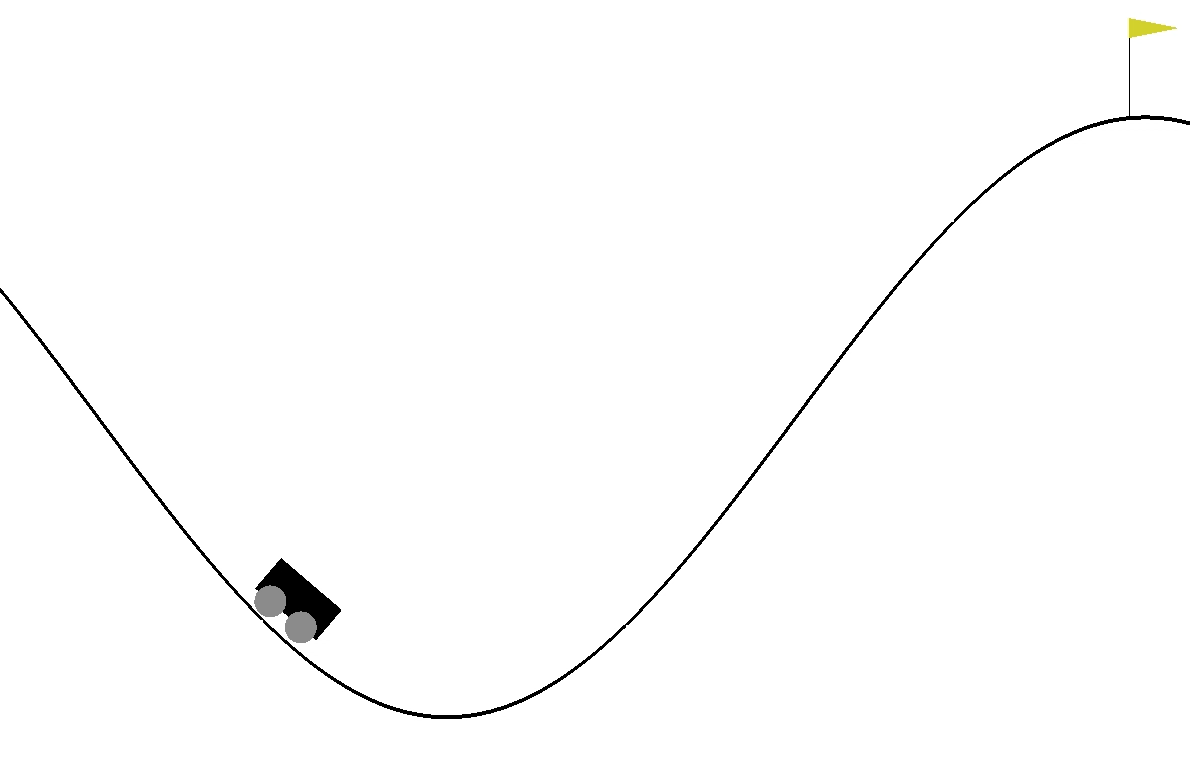
\includegraphics[width=7cm]{fig1.png}


    In the normal case, the car's aim is to reach the yellow flag where it will receive a reward.

    In the modified case, which interests us, the car driving agent was trained to reach a different location (unknown to us) by being provided a different reward signal. 

    We have access to:

    \begin{enumerate}
        \item the examples of the driving agent's actions over time
        \item the state before each decision was made, and
        \item a model of the environment
    \end{enumerate}

    Our goal is to uncover what the reward signal is.


    CRITICALLY: We assume that the actions we are observing are \textbf{optimal} for the reward function. In other words: We assume that the actions taken by the driver of the car are "perfect" so to speak, for the given reward function. 
    We then make inferences about possible reward functions, $R$, which satisfy the constraint that if an agent learns the optimal policy for $R$ it will exhibit the same behavior we observe in the driving examples provided. 


    \subsection{Identified issues}
    In any environment, with any observed action there exists multiple valid reward functions to explain the behavior. For example, in an environment which uniformly always gives 0 reward we can expect every policy in an environment with this $R$ to be "optimal". Such solutions to the IRL problem such as uniform reward functions are considered \emph{degenerate}.
    
    In order to select the "best" reward function $R$ is evaluated by how uniquely it describes the behavior exhibited. I.e. if $R$ can explain many different policies (think how the 0 reward solution explains every policy) then it is valued less.


    \subsection{Three Problem Areas}
    The paper highlights and provides solutions for 3 distinct types of environments and circumstances for IRL.
    \begin{enumerate} 
        \item Discrete environments where the policy is fully known (finite state space)
        \item Continuous environments where the policy is fully known (infinite state space)
        \item Continuous environments where you are only provided with a finite set of observed trajectories (infinite state space with limited information about the agent). This is the most realistic setting.
    \end{enumerate}

    \section{Medium Level}
    
    \subsection{Notation used by the paper}
    It's all pretty standard stuff:
    
    \begin{itemize}
        \item $S$ is a finite set of $N$ states
        \item $A = \{a_1, \dots, a_k\}$
        \item $P_{sa}(\cdot)$ are the state transition probabilities upon taking action $a$ in state $s$
        \item $\gamma \in [0,1)$ is the discount factor
        \item $R: S \mapsto \mathbb{R}$ is the reward function, bounded in absolute value by $R_{\max}$. They write the reward function as $R(s)$. 
        \item $\pi: S \mapsto A$ is a policy.
        \item $V^*(s) = \sup_\pi V^\pi (s)$ is the optimal value function
        \item $Q^*(s, a) = \sup_\pi Q^\pi (s, a)$ is the optimal Q-function
    \end{itemize}

    When looking at discrete problems, we represent the functions as \emph{vectors indexed by the state}.
    For example:
    $$\mathbf{R}[S_i] = \mbox{reward at $S_i$}$$  
    $$\mathbf{V}^\pi[S_i] = \mbox{value at $S_i$ while following policy $\pi$}$$  
    $$\mathbf{P}_a[S_i, S_j] = \mbox{starting in $S_i$, taking action $a$, probability of arriving in $S_j$ }$$  


    \section{Low Level}



\end{document}